\chapter{Implementation Concept}\label{implementation_concept}

The implementation is divided into the vector tile rendering process and the tile server. The following two sections describe the high level concept of both implementations.

\section{Vector Tile Rendering}

\paragraph{Import}
In the import phase data sources are imported into a spatial database and mapped to a database schema.

\paragraph{Export}
In the export phase a data style is applied to the database to produce vector tiles.

\paragraph{Data Style}
%\marginpar{The section \hyperref[data_style]{\emph{Data Style}} provides more details.}
The data style is a description of the vector tile structure and the SQL queries to fetch the data.

\begin{figure}[h]
  \centering
  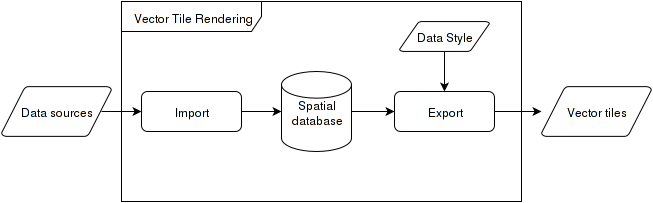
\includegraphics[scale=0.6]{images/vector_tile_rendering_squashed.png}
  \caption{Vector Tile Rendering Process}
\end{figure}

\section{Tile Server}

To display the vector tiles a tile server and a visual style is needed. There are two possibilities, which are described in the following two sections.

\paragraph{Visual Style}
The visual style defines how a feature class such as landuse actually gets displayed. In the case of landuse on could define the texture or the color of the border and area.


\subsection{Raster Tile Server}

The raster tile server makes it possible to display the vector tiles. It takes the visual style (CartoCSS\footnote{\url{https://github.com/mapbox/carto/blob/master/docs/latest.md}}) and the vector tiles as input. The renderer generates raster tiles of these inputs. When a raster tile is rendered, it is served by the webserver. Any GIS Software which supports raster tiles can consume the raster tiles served by the server.

\begin{figure}[h]

  \centering
  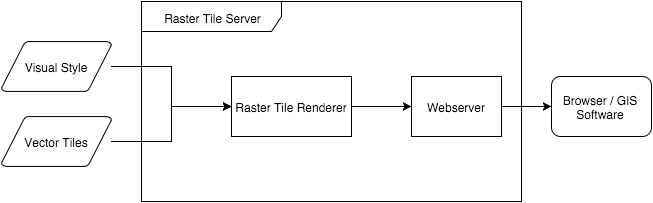
\includegraphics[width=1\textwidth]{images/raster_tile_server.png}
  \caption{Raster tile server}
\end{figure}

\subsection{Vector Tile Server}

The vector tile server in contrast to the raster tile variant directly serves the vector tiles to the client. The raster tiles are rendered on the client side using visual style. The advantage of this approach is more control over the user experience and that less server computing power is needed.

\begin{figure}[h]

  \centering
  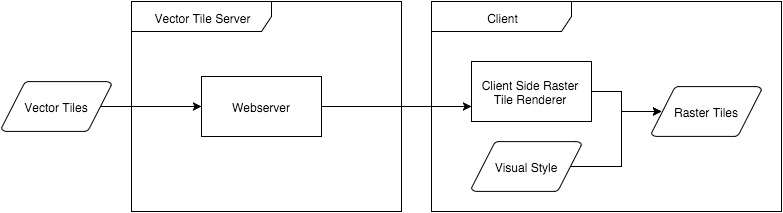
\includegraphics[width=1\textwidth]{images/vector_tile_server.png}
  \caption{Vector tile server}
\end{figure}

\newpage